\chapter{Исследовательский раздел}
\label{cha:research}
В данном разделе будет измерено время работы алгоритмов и сделаны выводы на основе полученных данных.
\section{Сравнительный анализ на основе замеров времени работы алгоритмов}
Для каждого из алгоритмов был проведён замер времени на матрицах размером от 100 до 1000 с шагом 100. Для каждого размера было проведено 10 повторений.
\par На рисунке 4.1 представлено сравнение времени для алгоритмов при чётных размерах матриц.
\begin{figure}
\centering
\begin{tikzpicture}[scale=1.5]
\begin{axis}[
axis lines = left,
xlabel = {Размер матрицы},
ylabel = {Время (секунды)},
legend pos=north west,
ymajorgrids=true
]
\addplot[color=red, mark=square] table[x index=0, y index= 1] {src/standardEven.txt}; 
\addplot[color=green, mark=square] table[x index=0, y index= 1] {src/winogradEven.txt}; 
\addplot[color=blue, mark=square] table[x index=0, y index= 1] {src/winoptimEven.txt}; 

\addlegendentry{Стандартный}
\addlegendentry{Алг. Винограда}
\addlegendentry{Оптимизированный алг.}

\end{axis}
\end{tikzpicture}
\caption{Сравнение времени работы алгоритмов на матрицах чётного размера}
\end{figure}

\par На рисунке 4.2 представлено сравнение времени работы для алгоритмов при нечётных размерах матриц.
\begin{figure}[H]
	\centering
	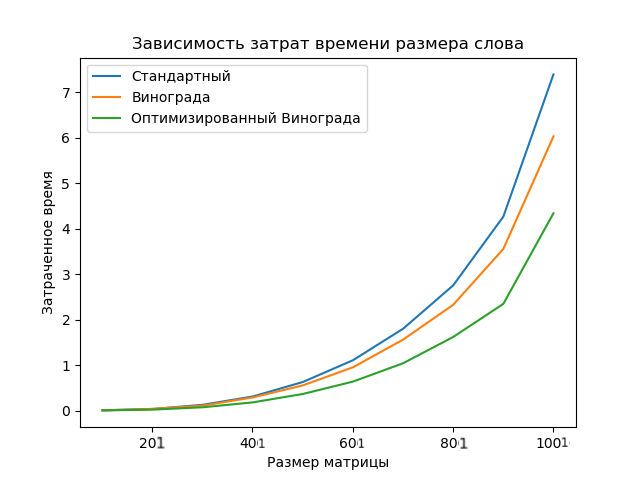
\includegraphics[width=0.7\linewidth]{src/odd}
	\caption{Сравнение времени работы алгоритмов на матрицах нечётного размера}
	\label{fig:odd}
\end{figure}

\par Из рисунков 4.2 и 4.1 видно, что для всех трёх алгоритмов асимптотика роста общая, однако как для чётных, так и для нечётных матриц оптимизированный алгоритм Винограда является самым быстрым, следующий по скорости алгоритм Винограда и самый медленный -- стандартный алгоритм умножения матриц.
\par Таким образом, данные, полученные в результате проведённых экспериментов подтверждают корректность рассчитанных ранее трудоёмкостей алгоритмов.
\par\textbf{Вывод.}
\par В итоге, можно сказать о том, что оптимизированный алгоритм Винограда является самым эффективным из рассмотренных.
